\documentclass{beamer}
\usepackage{Presentation}

\title[Compile-time Deadlock Detection in Rust]{Compile-time Deadlock Detection \\ in Rust using Petri Nets}
\author{Horacio Lisdero Scaffino}
\institute[FIUBA]{Facultad de Ingeniería\\Universidad de Buenos Aires}
\date{June 30, 2023}
% TWEAK THE FONT SIZE
\setbeamerfont{date}{size=\scriptsize}
% ADD LOGO
\logo{
\includegraphics[height=1.3cm]{FIUBA-Logo.png}}

\AtBeginSection[]
{
  \begin{frame}{Agenda}
  \footnotesize
    \tableofcontents[currentsection, currentsubsection]
  \end{frame}
}

\AtBeginSubsection[]
{
  \begin{frame}{Agenda}
  \footnotesize
    \tableofcontents[currentsection, currentsubsection]
  \end{frame}
}

\begin{document}

\begin{frame}
  \titlepage
\end{frame}

% REMOVE THE LOGO FROM NOW ON %
\logo{}

\begin{frame}{Agenda}
  \tableofcontents
\end{frame}

\section{Introduction}

\begin{frame}{A bird's-eye view of the tool}
  The Translator is the core component.
  The model checker and the Rust compiler, \emph{rustc}, are dependencies.

  \begin{figure}
    \centering
    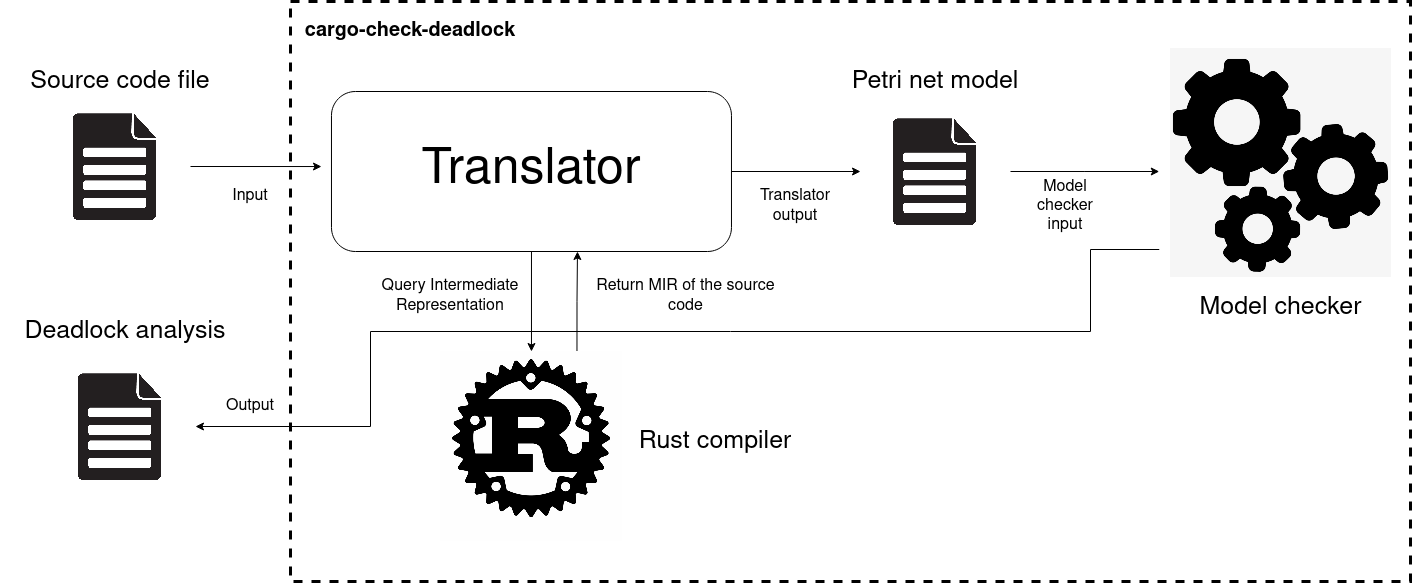
\includegraphics[width=\linewidth]{cargo-check-deadlock-logic-view.png}
  \end{figure}
\end{frame}

\section{Rust}

\subsection{What is Rust?}

\begin{frame}{What is Rust?}
  Rust is a multi-paradigm, general-purpose programming language that
  aims to provide developers with a safe and efficient way to write low-level code.

  \pause
  \vfill

  \begin{itemize}
    \item Memory-safe
    \item Compiled to machine code, no runtime needed
    \item High-level simplicity
    \item Low-level performance (on the same level as C or C++)
  \end{itemize}
\end{frame}

\begin{frame}{Brief timeline of Rust}
  \begin{description}
    \item [2007] Started as a side project by Graydon Hoare, a programmer at Mozilla
    \item [2009] Mozilla officially started sponsoring the project
    \item [2015] First stable version 1.0
    \item [2016] Mozilla releases Servo, a browser engine built with Rust
    \item [2019] \Rustinline{async}/\Rustinline{await} support stabilized
    \item [2021] The Rust Foundation is founded by AWS, Huawei, Google, Microsoft, and Mozilla
    \item [2021] The Android Open Source Project encourages the use of Rust for the SO components below the ART
    \item [2022] The Linux kernel adds support for Rust alongside C
    \item [2023] 8 years in a row the most loved programming language in the Stack Overflow Developer Survey
  \end{description}
\end{frame}

\begin{frame}{Memory safety}
  It achieves memory safety without using a garbage collector or reference counting.
  Instead, it uses the concept of \textbf{ownership} and \textbf{borrowing}.

  \vfill
  \pause

  It prevents a wide variety of error classes at compile-time:

  \begin{itemize}
    \item Double free
    \item Use after free
    \item Dangling pointers
    \item Data races
    \item Passing non-thread-safe variables
  \end{itemize}

  \vfill

  If a violation of the compiler rules is found, the program will simply not compile.
\end{frame}

\subsection{How does it look like?}

\begin{frame}[fragile]{Immutability by default}\
  \scriptsize
  In other languages, immutability is the exception or an afterthought (e.g. \texttt{const}-ness in C/C++).

  \begin{listing}
    \begin{minted}{Rust}
      fn main() {
        let x = 1; // Immutable by default
        x = x + 1;
      }
    \end{minted}
  \end{listing}

  \vfill
  The Rust compiler points out exactly where the error is and provides help on how to fix it.

  \begin{listing}
    \scriptsize
    \begin{Verbatim}[commandchars=\\\{\}]
      \textbf{\textcolor{red}{error[E0384]}: cannot assign twice to immutable variable `x`}
      --> src/main.rs:3:5
      |
    2 |     let x = 1;
      |         \textcolor{blue}{-}
      |         \textcolor{blue}{|}
      |         \textcolor{blue}{first assignment to `x`}
      |         \textcolor{blue}{help: consider making this binding mutable: `mut x`}
    3 |     x = x + 1;
      |     \textcolor{red}{^^^^^^^^^ cannot assign twice to immutable variable}
    \end{Verbatim}
  \end{listing}
\end{frame}

\begin{frame}[fragile]{Move semantics by default}
  Each value has only one owner.
  If a variable is passed to another function or assigned to a different variable, the owner of the value changes.

  \vfill

  \begin{listing}
    \begin{minted}{Rust}
      fn main() {
        let name = String::from("Alice");
        print_name(name);
        println!("The name is: {}", name); // Compilation error
      }
    
      fn print_name(name: String) {
          println!("Name: {}", name);
      }
    \end{minted}
  \end{listing}

  \vfill

  Values have copy semantics only if they are marked as \Rustinline{Copy}.
  This is the case for numbers by default. Compare this with the default in C++ vs the best practices.
\end{frame}

\begin{frame}[fragile]{Move semantics by default: Error message}
  \begin{listing}
    \raggedleft
    \tiny
    \begin{Verbatim}[commandchars=\\\{\}]
      \textbf{\textcolor{red}{error[E0382]}: borrow of moved value: `name`}
      --> src/main.rs:4:33
       |
     2 |     let name = String::from("Alice");
       |         \textcolor{blue}{---- move occurs because `name` has type `String`,
       |                                which does not implement the `Copy` trait}
     3 |     print_name(name);
       |                \textcolor{blue}{---- value moved here}
     4 |     println!("The name is: {}", name); // Compilation error
       |                               \textcolor{red}{^^^^ value borrowed here after move}
       |
     \textcolor{green}{note}: consider changing this parameter type in function `print_name` to borrow
     instead if owning the value isn't necessary
      --> src/main.rs:7:21
       |
     7 | fn print_name(name: String) \{
       |    \textcolor{blue}{----------}       \textcolor{green}{^^^^^^ this parameter takes ownership of the value}
       |    \textcolor{blue}{|}
       |    \textcolor{blue}{in this function}
       = \textbf{note}: this error originates in the macro `$crate::format_args_nl`
         which comes from the expansion of the macro `println` (in Nightly builds, run with -Z macro-backtrace for more info)
     help: consider cloning the value if the performance cost is acceptable
       |
     3 |     print_name(name.clone());
       |                    \textcolor{green}{++++++++}     
    \end{Verbatim}
  \end{listing}
\end{frame}

\begin{frame}[fragile]{Algebraic Data Types, aka enums with fields}
  \begin{listing}
    \begin{minted}[fontsize=\tiny, frame=none]{Rust}
      enum Shape {
        Circle { radius: f64 },
        Rectangle { width: f64, height: f64 },
        Triangle { base: f64, height: f64 },
      }
    
      fn main() {
          let shapes = vec![
              Shape::Circle { radius: 5.0 },
              Shape::Rectangle { width: 10.0, height: 8.0 },
              Shape::Triangle { base: 7.0, height: 4.0 },
          ];
      
          for shape in shapes {
              match shape {
                  Shape::Circle { radius } => {
                      let circle = Circle { radius };
                      // Do something with the circle...
                  },
                  Shape::Rectangle { width, height } => {
                      let rectangle = Rectangle { width, height };
                      // Do something with the rectangle...
                  },
                  Shape::Triangle { base, height } => {
                      let triangle = Triangle { base, height };
                      // Do something with the triangle...
                  },
              }
          }
      }
    \end{minted}
  \end{listing}
\end{frame}

\begin{frame}[fragile]{A more advanced match statement}
  A \Rustinline{match} statement works \emph{with} the type system,
  while a mere \Rustinline{if} can do anything and it is not bound to the type system.
  Match statements are always \emph{exhaustive}: They must handle all possibilities.

  \begin{listing}
    \begin{minted}[fontsize=\scriptsize, frame=none]{Rust}
      fn main() {
        let number = 42;
    
        match number {
            0 => println!("The number is zero"),
            1 | 2 | 3 => println!("The number is a small prime"),
            n @ 4..=9 => println!("The number is between 4 and 9: {n}"),
            n if is_even(n) => println!("The number is even: {n}"),
            n if is_odd(n) => println!("The number is odd: {n}"),
            _ => panic!("The number doesn't match any specific case!"),
        }
      }
    \end{minted}
  \end{listing}

  Python 3.10 introduced a similar feature (\href{https://peps.python.org/pep-0636/}{PEP 636}).
  Java 17 has a limited version of this (\href{https://openjdk.org/jeps/406}{JEP 406}).
\end{frame}

\begin{frame}[fragile]{Modeling data in Rust}
  \begin{itemize}
    \item Leverage the type system in your favor
    \item Make invalid states unrepresentable
    \item Define new types for the entities in your domain
    \item Use enums when variables can take different values
  \end{itemize}

  \begin{multicols}{2}
    \begin{listing}
      \begin{minted}[fontsize=\scriptsize, frame=none]{Rust}
        struct FakeCat {
          alive: bool,
          hungry: bool,
        }
      \end{minted}
    \end{listing}

    \begin{listing}
      \begin{minted}[fontsize=\scriptsize, frame=none]{Rust}
        enum RealCat {
          Alive { hungry: bool },
          Dead,
        }
      \end{minted}
    \end{listing}
  \end{multicols}
  
  By directly modeling the business domain with Rust's expressive type system,
  the compiler is able to verify the business logic and
  we catch more errors at compile-time.
\end{frame}

\begin{frame}[fragile]{Error handling with Result}
  \begin{listing}
    \begin{minted}[fontsize=\tiny, frame=none]{Rust}
      use std::fs::File;
      use std::io::Read;
      // This definition is part of the standard library
      // It does not need to be imported
      enum Result<T, E> {
        Ok(T),
        Err(E),
      }  
      
      fn read_file_contents(path: &str) -> Result<String, std::io::Error> {
          let mut file = File::open(path)?;
          let mut contents = String::new();
          file.read_to_string(&mut contents)?;
          Ok(contents)
      }
      
      fn main() {
          let file_path = "example.txt";
          let result = read_file_contents(file_path);
      
          match result {
              Ok(contents) => {
                  println!("File contents:\n{}", contents);
              }
              Err(error) => {
                  eprintln!("Error reading file: {}", error);
              }
          }
      }      
    \end{minted}
  \end{listing}
\end{frame}

\begin{frame}[fragile]{The enum Option: No need for null pointers}
  \begin{listing}
    \begin{minted}[fontsize=\scriptsize, frame=none]{Rust}
      // This definition is part of the standard library
      // It does not need to be imported
      pub enum Option<T> {
        None,
        Some(T),
      }

      fn main() {
        let mut list = vec![1, 2, 3, 4, 5];
    
        while let Some(element) = list.pop() {
            println!("Popped element: {}", element);
        }
        // List::pop() returned `None`
        println!("List is empty!");
      }
    \end{minted}
  \end{listing}
\end{frame}

\begin{frame}[fragile]{No OOP: Just structs with methods}
  \begin{listing}
    \begin{minted}[fontsize=\scriptsize, frame=none]{Rust}
      struct Rectangle {
          width: u32,
          height: u32,
      }
      
      impl Rectangle {
          fn new(width: u32, height: u32) -> Rectangle {
              Rectangle { width, height }
          }
      
          fn area(&self) -> u32 {
              self.width * self.height
          }
      
          fn is_square(&self) -> bool {
              self.width == self.height
          }
      
          fn double_size(&mut self) {
              self.width *= 2;
              self.height *= 2;
          }
      }
    \end{minted}
  \end{listing}
\end{frame}

\begin{frame}[fragile]{Define traits to share an interface}
  \begin{listing}
    \begin{minted}[fontsize=\tiny, frame=none]{Rust}
      trait Container {
        fn get_value(&self);
      }
      
      struct Storage {
          value: i32,
      }
      
      impl Container for Storage {
          fn get_value(&self) {
              println!("Value: {}", self.value);
          }
      }
      
      impl PartialEq for Storage {
          fn eq(&self, other: &Self) -> bool {
              self.value == other.value
          }
      }
      
      impl std::fmt::Display for Storage {
          fn fmt(&self, f: &mut std::fmt::Formatter) -> std::fmt::Result {
              write!(f, "Value: {}", self.value)
          }
      }
    \end{minted}
  \end{listing}
\end{frame}

\begin{frame}[fragile]{Nearly everything is an expression as in Lisp}
  \begin{listing}
    \begin{minted}[fontsize=\scriptsize, frame=none]{Rust}
      fn main() {
        let numbers = vec![1, 2, 3, 4, 5];
    
        let sum_of_squares: i32 = numbers
            .iter()
            .fold(0, |acc, x| acc + x * x);
    
        let result = if sum_of_squares > 50 {
            "Sum of squares is greater than 50"
        } else {
            "Sum of squares is not greater than 50"
        };
    
        println!("Result: {}", result);
      }
    \end{minted}
  \end{listing}
\end{frame}

\begin{frame}[fragile]{Generics}
  \begin{listing}
    \begin{minted}[fontsize=\scriptsize, frame=none]{Rust}
      struct Pair<T, U> {
        first: T,
        second: U,
      }
    
      impl<T, U> Pair<T, U> {
          fn new(first: T, second: U) -> Self {
              Pair { first, second }
          }
      
          fn get_first(&self) -> &T {
              &self.first
          }
      
          fn get_second(&self) -> &U {
              &self.second
          }
      }
    \end{minted}
  \end{listing}
\end{frame}

\begin{frame}[fragile]{Lifetimes}
  \begin{listing}
    \begin{minted}[fontsize=\tiny, frame=none]{Rust}
      struct StringHolder<'a> {
        value: &'a str,
      }
      
      impl<'a> StringHolder<'a> {
          fn new(value: &'a str) -> Self {
              StringHolder { value }
          }
      
          fn get_value(&self) -> &'a str {
              self.value
          }
      }
      
      fn main() {
          let input_string = String::from("Hello, lifetimes!");
      
          let holder;
          {
              let local_string = String::from("Local string");
              holder = StringHolder::new(local_string.as_str());
              println!("Holder value: {}", holder.get_value());
          }
      
          println!("Input string: {}", input_string);
          println!("Holder value: {}", holder.get_value());
      }
    \end{minted}
  \end{listing}
\end{frame}

\begin{frame}[fragile]{Lifetimes: Error message}
  \begin{listing}
    \raggedleft
    \tiny
    \begin{Verbatim}[commandchars=\\\{\}]
      \textbf{\textcolor{red}{error[E0597]}: `local_string` does not live long enough}
      --> src/main.rs:21:36
       |
    20 |         let local_string = String::from("Local string");
       |             \textcolor{blue}{------------ binding `local_string` declared here}
    21 |         holder = StringHolder::new(local_string.as_str());
       |                                    \textcolor{red}{^^^^^^^^^^^^^^^^^^^^^ borrowed value does not}
       |                                                                 \textcolor{red}{live long enough}
    22 |         println!("Holder value: {}", holder.get_value());
    23 |     \}
       |     \textcolor{blue}{- `local_string` dropped here while still borrowed}
    ...
    26 |     println!("Holder value: {}", holder.get_value());
       |                                \textcolor{blue}{------------------ borrow later used here}
    
    \textbf{For more information about this error, try `rustc --explain E0597`.}
    \end{Verbatim}
  \end{listing}
\end{frame}

\begin{frame}[fragile]{Only one active mutable reference at any given time}
  \begin{listing}
    \begin{minted}[fontsize=\tiny, frame=none]{Rust}
      struct Item {
        value: i32,
      }
      
      fn main() {
          let mut item = Item { value: 42 };
      
          let reference1 = &mut item; // First mutable reference
          let reference2 = &mut item; // Second mutable reference - COMPILATION ERROR
      
          reference1.value += 1;
          reference2.value += 1;
      
          println!("Reference 1: {}", reference1.value);
          println!("Reference 2: {}", reference2.value);
      }
    \end{minted}
  \end{listing}

  \begin{listing}
    \tiny
    \begin{Verbatim}[commandchars=\\\{\}]
      \textbf{\textcolor{red}{error[E0499]}: cannot borrow `item` as mutable more than once at a time}
      --> src/main.rs:9:22
       |
    8  |     let reference1 = &mut item; // First mutable reference
       |                      \textcolor{blue}{--------- first mutable borrow occurs here}
    9  |     let reference2 = &mut item; // Second mutable reference - COMPILATION ERROR
       |                      \textcolor{red}{^^^^^^^^^ second mutable borrow occurs here}
    10 |
    11 |     reference1.value += 1;
       |     \textcolor{blue}{--------------------- first borrow later used here}
    
    \textbf{For more information about this error, try `rustc --explain E0499`.}
    \end{Verbatim}
  \end{listing}
\end{frame}

\begin{frame}[fragile]{A mutable reference is allowed only if no immutable references are present}
  \begin{listing}
    \begin{minted}[fontsize=\tiny, frame=none]{Rust}
      fn main() {
        let mut item = 42;
    
        let reference1 = &item; // First mutable reference
        let reference2 = &mut item; // Second mutable reference - COMPILATION ERROR
    
        if *reference1 == 1 {
            println!("Item is set to one");
        }
        *reference2 += 1;
    
        println!("Reference 1: {}", reference1);
        println!("Reference 2: {}", reference2);
      }
    \end{minted}
  \end{listing}

  \begin{listing}
    \tiny
    \begin{Verbatim}[commandchars=\\\{\}]
      \textbf{\textcolor{red}{error[E0502]}: cannot borrow `item` as mutable because it is also borrowed as immutable}
      --> src/main.rs:5:22
       |
     4 |     let reference1 = &item; // First mutable reference
       |                      \textcolor{blue}{----- immutable borrow occurs here}
     5 |     let reference2 = &mut item; // Second mutable reference - COMPILATION ERROR
       |                      \textcolor{red}{^^^^^^^^^ mutable borrow occurs here}
     6 |
     7 |     if *reference1 == 1 \{
       |        \textcolor{blue}{----------- immutable borrow later used here}
    \end{Verbatim}
  \end{listing}
\end{frame}

\subsection{Why Rust?}

\begin{frame}{Memory safety is critical for reliability and security}
  Empirical investigations have concluded that around 70\% of the vulnerabilities found in
  large C/C++ codebases are due to memory handling errors. This high figure can be observed in
  projects such as:

  \begin{itemize}
    \item Android Open Source Project \cite{memory-bugs-android},
    \item the Bluetooth and media components of Android \cite{memory-bugs-android-media-bluetooth},
    \item the Chromium Projects behind the Chrome web browser \cite{memory-bugs-chrome},
    \item the CSS component of Firefox \cite{memory-bugs-firefox},
    \item iOS and macOS \cite{memory-bugs-ios-macos},
    \item Microsoft products \cite{miller-security-microsoft2019, memory-bugs-microsoft},
    \item Ubuntu \cite{memory-bugs-ubuntu}
  \end{itemize}
\end{frame}

\begin{frame}{Rust adoption is increasing fast}
  \scriptsize
  \begin{itemize}
    \item The Android Open Source Project encourages
          the use of Rust for the SO components
          below the ART \cite{stoep2021}.
    \item The Linux kernel introduces in version 6.1 official tooling
          support for programming components in Rust \cite{corbet2022,desimone2022}.
    \item At Mozilla, the Oxidation project was created in 2015
          to increase the usage of Rust in Firefox and related projects.
          As of March 2023, the lines of code in Rust represent more than
          10\% of the total in Firefox Nightly \cite{mozilla-oxidation}.
    \item At Meta, the use of Rust as a development language server-side
          is approved and encouraged since July 2022 \cite{garcia2022}.
    \item At Cloudflare, a new HTTP proxy in Rust was built from scratch
          to overcome the architectural limitations of NGINX,
          reducing CPU usage by 70\% and memory usage by 67\% \cite{wu2022}.
    \item At Discord, reimplementing a crucial service
          in Rust provided great benefits in performance
          and solved a performance penalty due to the garbage collection in Go \cite{howarth2020}.
    \item At npm Inc., the company behind the npm registry, Rust allowed scaling CPU-bound services
          to more than 1.3 billion downloads per day \cite{rust-npm-case-study}.
    \item A study of Rust-based code found it runs so efficiently
          that it uses half as much electricity as a similar program written in Java,
          a language commonly used at AWS \cite{pereira2017energy}.
  \end{itemize}
\end{frame}

\begin{frame}{The tooling is great and works out of the box}
  \begin{itemize}
    \item \href{https://doc.rust-lang.org/stable/cargo/}{cargo},
          the official package manager: Format, build, test, lint, update, and publish packages.
    \pause
    \item \href{https://doc.rust-lang.org/book/ch11-00-testing.html}{Test harness}
          for unit tests, integration tests, and tests in documentation comments (doctests).
          No third-party libraries needed.
    \pause
    \item An official public registry for Rust packages (called ``crates''): \url{https://crates.io/}.
    \pause
    \item Automatic generation of a static website from the doc comments of the project.
          It is published automatically to \url{https://docs.rs/}.
    \pause
    \item An official linter included with the default installation that catches even more errors
          and spots non-idiomatic code: \href{https://github.com/rust-lang/rust-clippy}{clippy}.
    \pause
    \item Integration with git, GitHub, VSCode, IntelliJ is great and easy to use.
    \pause
    \item A new stable compiler release every 6 weeks \cite{albini2019}.
  \end{itemize}
\end{frame}

\section{Petri nets}

\subsection{What is a Petri net?}

\begin{frame}{Informal definition}
  A Petri net is a mathematical modeling tool
  used to describe and analyze the behavior of concurrent systems.
  It provides a graphical representation of the system's state and its transitions,
  allowing for visual and formal analysis of complex processes.
  
  \begin{figure}[!htb]
    \centering
    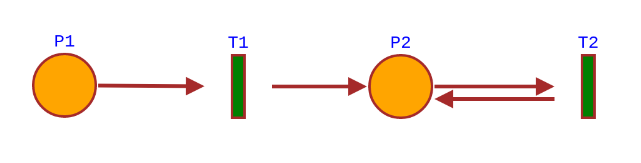
\includegraphics[width=0.8\linewidth]{petri-net-formal-example.png}
  \end{figure}

  \scriptsize
  \begin{itemize}
    \item Places: Represent states in the system (\emph{circles})
    \item Transitions: Represent usually events or actions that occur in the system (\emph{rectangles})
    \item Tokens: Marks inside of places that are created
          and consumed by transitions (\emph{points inside of places})
  \end{itemize}
  
  \vfill
\end{frame}

\begin{frame}{Mathematical definition}
  A Petri net is a 5-tuple, $ PN = (P, T, F, W, M_{0}) $ where:

  \begin{quote}
        $ P = \{ p_1, p_2, \dots, p_m \} $ is a finite set of places,\\
        $ T = \{ t_1, t_2, \dots, t_n \} $ is a finite set of transitions,\\
        $ F \subseteq (P \times T) \cup (T \times P) $ is a set of arcs (flow relation),\\
        $ W: F \rightarrow \{1, 2, 3, ... \} $ is a weight function for the arcs,\\
        $ M_{0}: P \rightarrow \{0, 1, 2, 3, .... \} $ is the initial marking,\\
        $ P \cap T = \varnothing $ and $ P \cup T \neq \varnothing $
  \end{quote}

  The graph is by definition \emph{bipartite}.
  There can only be edges:
  \begin{itemize}
    \item from places to transitions or
    \item from transitions to places
  \end{itemize}

\end{frame}

\begin{frame}{Transition firing rule}
  \begin{figure}[!htb]
    \centering
    \includesvg[width=0.9\linewidth]{petri-net-transition-example.svg}
  \end{figure}
\end{frame}

\subsection{Examples}

\begin{frame}{Vending machine}
  \scriptsize
  This is a finite-state machine (FSM), a subclass of Petri nets.

  \begin{figure}
    \centering
    \includesvg[width=\linewidth]{state-machine-example.svg}
  \end{figure}
\end{frame}

\begin{frame}{Parallel activities: Fork/Join}
  \scriptsize
  This is a marked graph (MG), a subclass of Petri nets.
  Observe the concurrency between Task 1 and Task 2.
  This cannot be modeled by a single finite-state machine. 

  \begin{figure}
    \centering
    \includesvg[width=0.8\linewidth]{parallel-activities-example.svg}
  \end{figure}
\end{frame}

\begin{frame}{Communication protocols: Send with ACK}
  \scriptsize
  A simple protocol in which Process 1 sends messages to Process 2 and
  waits for an acknowledgment to be received before continuing.
  For simplicity, no timeout mechanism was included.

  \begin{figure}
    \centering
    \includesvg[width=0.90\linewidth]{communication-protocols-example.svg}
  \end{figure}
\end{frame}

\begin{frame}{Synchronization control: Readers and writers}
  \scriptsize
  A Petri net system with k processes that either read or write a shared value.

  \begin{itemize}
    \item If one process writes, then no process may read.
    \item If a process is reading, then no process may write.
    \item There can only be zero or one process writing at any given time.
  \end{itemize}

  \begin{figure}
    \centering
    \includesvg[width=0.9\linewidth]{readers-writers-example.svg}
  \end{figure}
\end{frame}

\subsection{Why Petri nets?}

\begin{frame}{Reachability analysis}
  Petri nets can be analyzed using formal methods to conclude whether the net can reach
  a deadlock or not. There is a notion of liveness analogous to the one found in computer systems.

  \vfill
  \pause

  Several model checkers are being developed and
  there is even a Model Checking Contest that takes place every year.
  State-of-the-art tools can handle Petri net models
  with more than \textbf{70 000 transitions} and \textbf{one million places}.

  \vfill
  \pause

  Translating source code to a Petri net has been done before for other programming languages
  \cite{kavi2002modeling,moshtaghi2001} and also for Rust \cite{meyer2020, zhang2022deadlocks}.
  The difficulty lies in supporting more synchronization primitives
  than simple mutexes and translating code from real-world applications.
\end{frame}

\section{Translation}

\begin{frame}{Compilation stages in \emph{rustc}}
  \scriptsize

  \begin{itemize}
    \item Lexing: The source text is turned into a stream of atomic source code units known as tokens.
    \pause
    \item Parsing: The stream of tokens is converted into an \textbf{Abstract Syntax Tree}.
    \pause
    \item High-level Intermediate Representation (HIR):
    \begin{itemize}
      \scriptsize
      \setbeamertemplate{itemize items}[circle]
      \item Desugar loops: \Rustinline[fontsize=\scriptsize]{while} and \Rustinline[fontsize=\scriptsize]{for} to simple \Rustinline[fontsize=\scriptsize]{loop}.
      \item Type inference: The automatic detection of a type of an expression.
      \item Trait solving: Ensuring that each implementation block (\Rustinline[fontsize=\scriptsize]{impl}) points to a valid trait.
      \item Type checking.
    \end{itemize}
    \pause
    \item Mid-level Intermediate Representation (MIR): 
    \begin{itemize}
      \scriptsize
      \setbeamertemplate{itemize items}[circle]
      \item Checking of exhaustiveness of pattern matching.
      \item Desugar method calls to function calls\\
                    (\Rustinline[fontsize=\scriptsize]{x.method(y)} becomes \Rustinline[fontsize=\scriptsize]{Type::method(&x, y)}).
      \item Add implicit dereferencing operations.
      \item Borrow checking.
    \end{itemize}
    \pause
    \item Code generation:
    \begin{itemize}
      \scriptsize
      \setbeamertemplate{itemize items}[circle]
      \item Rust relies on LLVM as a backend.
      \item It leverages many optimizations of the LLVM intermediate representation.
      \item LLVM takes over from this point on.
      \item At the end, object files are linked to create an executable.
    \end{itemize}
  \end{itemize}
\end{frame}

\subsection{MIR}

\begin{frame}[fragile]{Hello World in MIR}
  \tiny
  BB means ``basic block''. Each one is formed by statements and one terminator statement.
  The terminator statement is the only place where the control flow can jump to another basic block.

  \begin{listing}
    \begin{minted}[fontsize=\scriptsize, frame=none]{Rust}
      fn main() -> () {
          let mut _0: ();                     
          let _1: ();                         
          let mut _2: std::fmt::Arguments<'_>;
          let mut _3: &[&str];                
          let mut _4: &[&str; 1];             
      
          bb0: {
              _4 = const _;                    
              _3 = _4 as &[&str] (Pointer(Unsize));
              _2 = Arguments::<'_>::new_const(move _3) -> bb1;
          }
      
          bb1: {
              _1 = _print(move _2) -> bb2;
          }
      
          bb2: {
              return;
          }
      }      
    \end{minted}
  \end{listing}
\end{frame}

\begin{frame}{MIR as a graph that shows the flow of execution}
  \scriptsize
  The MIR is a form of control flow graph (CFG) used in compilers.
  In this form, the translation to a Petri net becomes evident.

  \begin{figure}[!htb]
    \centering
    \includesvg[width=0.50\linewidth]{mir-cfg-example.svg}
  \end{figure}
\end{frame}

\subsection{Modeling threads}

\begin{frame}[fragile]{Example program}
  Let's consider a trivial program that spawns a thread that does nothing
  and immediately joins it.

  \vfill

  \begin{listing}
    \begin{minted}[fontsize=\scriptsize, frame=none]{Rust}
      fn main() {
        let thread_join_handle = std::thread::spawn(move || {
            // some work here
        });
        // some work here
        let _res = thread_join_handle.join();
      }   
    \end{minted}
  \end{listing}

  \vfill
  
  \begin{itemize}
    \item \Rustinline{std::thread::spawn} should create an additional token
          that models the program counter of the second thread.
    \item The joining thread should wait until the spawned thread finishes.
  \end{itemize}
\end{frame}

\begin{frame}{Petri net model for a thread}
  \begin{figure}
    \centering
    \includesvg[height=0.85\textheight]{multithreading-example.svg}
  \end{figure}
\end{frame}

\subsection{Modeling mutexes}

\begin{frame}[fragile]{Example program}
  Consider a simple program that locks a mutex twice.
  The second lock operation will deadlock
  because the lock handle returned by the first call to \Rustinline{std::sync::Mutex::lock}
  is not dropped until it falls out of scope.

  \vfill

  \begin{listing}
    \begin{minted}[fontsize=\scriptsize, frame=none]{Rust}
      fn main() {
        let data = std::sync::Mutex::new(0);
        let _d1 = data.lock();
        let _d2 = data.lock(); // cannot lock, since d1 is still active
      }
    \end{minted}
  \end{listing}

  \vfill
  
  \begin{itemize}
    \item There should be a single place that models the mutex.
    \item Locking the mutex is taking the token from the mutex place.
    \item Unlocking the mutex is setting the token back in the mutex place.
  \end{itemize}
\end{frame}

\begin{frame}{Petri net model for a mutex}
  \begin{figure}
    \centering
    \includesvg[height=0.85\textheight]{mutex-example.svg}
  \end{figure}
\end{frame}

\subsection{Modeling condition variables}

\begin{frame}{How to model a condition variable}
  \begin{figure}
    \centering
    \includesvg[height=0.85\textheight]{condition-variable-model.svg}
  \end{figure}
\end{frame}

\begin{frame}[fragile]{Example program}
  We have to use a very simple example program to keep the net small.
  In this case, the thread is trying to notify itself, which leads to a lost signal.

  \begin{listing}
    \begin{minted}[fontsize=\scriptsize, frame=none]{Rust}
      fn main() {
        let mutex = std::sync::Mutex::new(false);
        let cvar = std::sync::Condvar::new();
        let mutex_guard = mutex.lock().unwrap();
        cvar.notify_one();
        let _result = cvar.wait(mutex_guard);
      }     
    \end{minted}
  \end{listing}

  \begin{itemize}
    \item The model for the condition variable should appear in the Petri net.
    \item The notify place should be set.
    \item But the signal gets consumed because \Rustinline{std::sync::Condvar::wait} was not called.
  \end{itemize}
\end{frame}

\begin{frame}{Petri net model for the example program}
  \begin{figure}
    \centering
    \includesvg[height=0.85\textheight]{condition-variable-example.svg}
  \end{figure}
\end{frame}

\section{Bibliography}

\begin{frame}[allowframebreaks]{Bibliography}
  \tiny
  \bibliographystyle{ieeetr}
  \bibliography{
    ../Bibliography/Articles.bib,
    ../Bibliography/Blogs.bib,
    ../Bibliography/Books.bib,
    ../Bibliography/Conferences.bib,
    ../Bibliography/Proceedings.bib
  }
\end{frame}

\section{Additional resources}

\begin{frame}{Resources to learn Rust}
  \begin{itemize}
    \item \href{https://doc.rust-lang.org/stable/book/}{The Rust Book}:
          Available online and locally with the default Rust installation.
    \item \href{https://doc.rust-lang.org/rust-by-example/}{Rust by Example}:
          Another official book with a more practical approach.
    \item \href{https://github.com/rust-lang/rustlings}{Rustlings}:
          Small exercises to get you used to reading and writing Rust code! 
    \item \href{https://google.github.io/comprehensive-rust/}{Comprehensive Rust}:
          A three-day Rust course developed by the Android team.
    \item \href{https://learn.microsoft.com/en-us/training/paths/rust-first-steps/}{Take your first steps with Rust}:
          A simple course on Microsoft Learn.
    \item \href{https://www.youtube.com/watch?v=MsocPEZBd-M}{Rust Programming Course for Beginners} by freeCodeCamp.org.
    \item \href{https://www.youtube.com/\@NoBoilerplate/videos}{No Boilerplate}:
          A Youtube channel mainly dedicated to topics connected with Rust. Some ideas were used for this presentation.
  \end{itemize}
\end{frame}

\begin{frame}{Online Petri net simulators}
  \begin{itemize}
    \item A simple simulator by Igor Kim can be found on \url{https://petri.hp102.ru/}.
          A tutorial video on Youtube and example nets are included in the tool.
    \item A complement to this is a series of interactive tutorials by Prof. Wil van der Aalst
          at the University of Hamburg. These tutorials are Adobe Flash Player files (with extension \texttt{.swf})
          that modern web browsers cannot execute.
          Luckily, an online Flash emulator like the one found on \url{https://flashplayer.fullstacks.net/?kind=Flash_Emulator}
          can be used to upload the files and execute them.
    \item Another online Petri net editor and simulator is \url{http://www.biregal.com/}.
          The user can draw the net, add the tokens, and then manually fire transitions.
  \end{itemize}
\end{frame}

\begin{frame}{}
  \huge
  \centering
  Questions?


  \vfill
  \raggedright
  \normalsize
  \textbf{Links}
  
  \scriptsize

  \begin{description}
    \item [Thesis] \url{https://github.com/hlisdero/thesis}
    \item [Tool] \url{https://github.com/hlisdero/cargo-check-deadlock}
    \item [Prasentation] \url{https://github.com/hlisdero/thesis/tree/main/presentation}
    \item [Published crate] \url{https://crates.io/crates/cargo-check-deadlock}
  \end{description}
\end{frame}

\end{document}
